\documentclass[UTF8]{article}
\usepackage{ctex}
\usepackage{geometry}
\usepackage{amsmath}
\usepackage{amssymb}
\usepackage{amsfonts}
\usepackage{bm}
\usepackage{graphicx}
\usepackage{listings}

\renewcommand{\baselinestretch}{1.5}


\title{\vspace{-5em}数据仓库与数据挖掘 大作业}
\author{\vspace{-5em}软博22 管浩荃 2022312726, 软硕221 陈子陵 2022213872}
\date{}
\geometry{a4paper, left=3.18cm, right=3.18cm, top=3.18cm, bottom=3.18cm}

\begin{document}
\maketitle
\section{数据处理}
可以发现,为了基于脓毒症患者在24小时观测窗口的生命体征数据预测观测窗口结束之后6小时是否死亡,首先需要保证患者在观测窗口内的数据是干净且有效的。因此,需要对时间序列做出相应的处理。

\subsection{数据缺失值处理}
对于数据的缺失值,在处理的过程中可以发现有空缺的行较少,因此将此类数据全部去除。事实上,对于训练数据集而言,去除缺失值前后的数据集维度分别为$(265030,7)$和$(214265,7)$。被去除的行数相比于总行数的比例并不高。

\subsection{异常值处理}
通过对数据集内数据的观察,可以发现数据集中有一些不符合实际的极端数值,即病人的生命体征不可能处于该值下。因此,我们将其识别为异常值。

结合实际情况和文档给出的健康范围,我们去除了如下数据所在的数据行:呼吸率超过60;氧饱和度低于50;平均动脉压$<0$或$>180$。

同时注意到,呼吸率为$0$有可能有两种情况。其一,在数据收集的过程中,由于机器故障或传输问题,呼吸率并没有被成功接收。其二,可能病人在该时间点已停止呼吸,呼吸率为$0$是病人的真实情况。基于如上考虑,在数据处理的过程中只对呼吸率过高的数据所在行进行处理。

\subsection{不等长序列处理}\label{subsect:icd9}
可以发现,对于每个病人,其时间序列虽然都处于24小时的观测窗口之内,但是序列的长度并不相同。为保证能使用batch进行模型的训练,并且规范所有病人的生命体征数据序列长短以优化模型效果,拟对所有病人的序列进行如下处理。

\begin{enumerate}
    \item 假如原本序列长度超过20,那么只保留最后的20个时刻;
    \item 假如原本序列长度不足20,那么将最后一个时刻的数据进行重复。
\end{enumerate}

\subsection{规范化}
由于患者的生命体征数据所处的范围并不相同,因此不进行规范化可能会使得每个字段对模型的影响有极大的差别。因此,需要将所有的数据进行规范化,以平衡四个字段的影响。由此,对于四个字段heartrate,resprate,map,o2sat中的每一个,都进行如下处理(下面用attr表示前述任意字段):

\begin{enumerate}
    \item[1] 首先,在数据集中加入了新字段attr\_DELTA表示差分后的结果。这是出于两个原因:(1)、体征稳定的病人更加安全;(2)、病人本身有自身体质,比如说自然状态下的某些病人心率就偏低,所以用差分后的数据帮助学习。
    \item[2] 而后,在数据集中加入了新字段attr\_ERR表示异常程度:为了利用说明文档给出的正常值范围,新增该字段表示属性偏离正常范围的程度。
        \begin{enumerate}
            \item[2.1] 注意到许多时候病人指标会在正常范围边缘(比如氧饱和度在$94\sim96$之间波动而正常边界是95),所以不是简单的0/1表示是否正常而是用连续值,指标偏离正常范围越多那么该字段数值就越大。
            \item[2.2] 根据背景知识,氧饱和度指标是越高越好(100是最好的)。
        \end{enumerate}
    \item[3] 将attr从原始数据改为数据离正常范围中间值的距离。这是因为原始数据太小和太大(比如心率过低和过高)都是不利生存的表现,做这一步处理之后,数值就是越小越好,方便学习。
    \item[4] 对数值型数据的规范化流程,使用正常值范围对数据进行标准化,将正常值的范围变为$[0,1]$。这样可以确保模型正常学习。
\end{enumerate}

处理后的部分字段分布图所示。其中,左右两图分别表示标签为0和1的训练集数据。在对数据集进行预处理后,可以发现数据大小和生存情况的关系更加直观。

\begin{figure}[h]
    \centering
    \begin{minipage}{.43\linewidth}
        \centering
        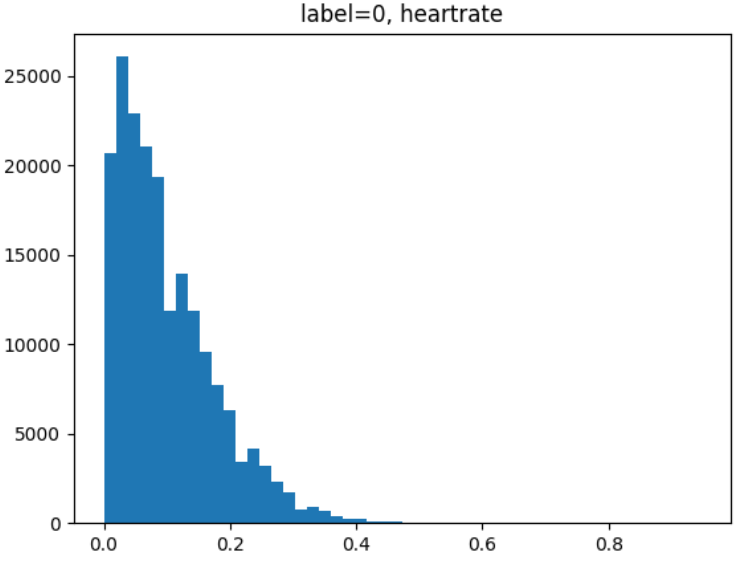
\includegraphics[width=\linewidth]{../source_code/attr_0.png}
    \end{minipage}
    \begin{minipage}{.43\linewidth}
        \centering
        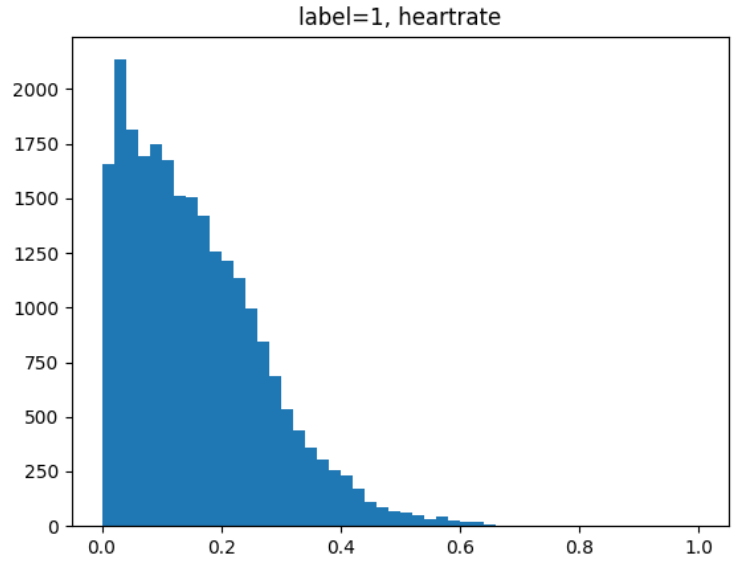
\includegraphics[width=\linewidth]{../source_code/attr_1.png}
    \end{minipage}
\end{figure}

\begin{figure}[h]
    \centering
    \begin{minipage}{.43\linewidth}
        \centering
        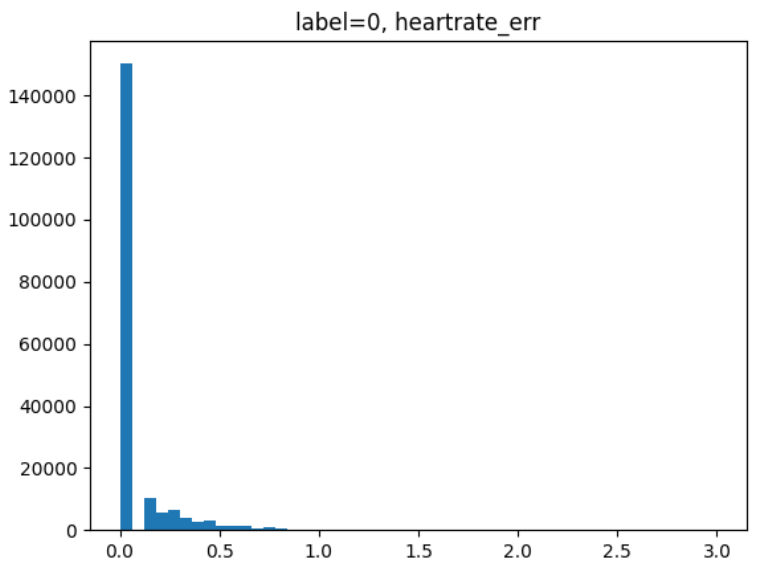
\includegraphics[width=\linewidth]{../source_code/err_0.png}
    \end{minipage}
    \begin{minipage}{.43\linewidth}
        \centering
        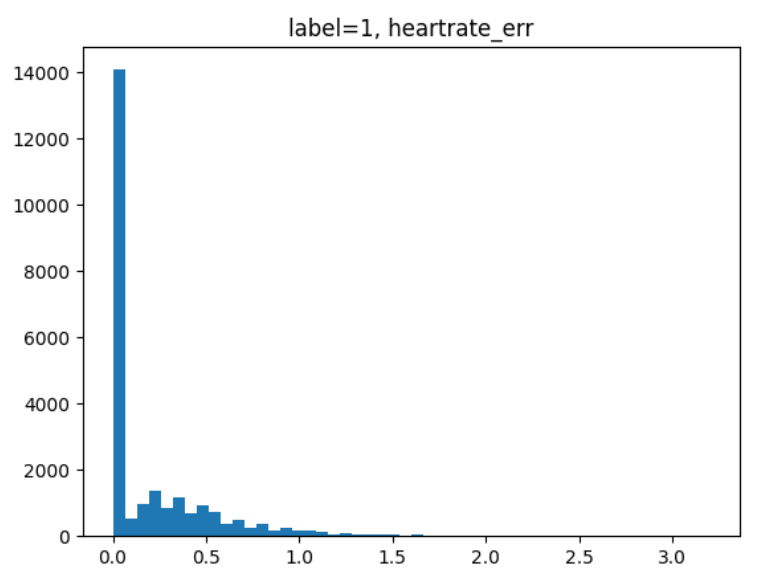
\includegraphics[width=\linewidth]{../source_code/err_1.png}
    \end{minipage}
\end{figure}

\section{回归模型与实验结果}
本节中,我们选择了传统RNN,GRU,LSTM进行回归预测,并用Accuracy、F1分析预测结果,并给出了ROC曲线和混淆矩阵。这是因为Accuracy可以反映出模型在整个数据集上的表现,F1可以反映出模型在正样本和负样本上的综合表现,ROC曲线和混淆矩阵可以体现出模型预测标签和实际标签之间的关系。

\subsection{传统RNN}
我们使用torch.nn.RNN作为模型对数据集进行训练。可以发现,对于传统RNN,随着epoch轮数的增进,Accuracy和F1 Score变化不明显。这说明RNN对数据集的建模能力不强。Accuracy虽然达到了0.91,但是其仍低于GRU和LSTM的结果,且这是因为数据集中有很多标签为0的数据。同时,F1 Score只有0.4左右,这是较低的。

\begin{figure}[h]
    \centering
    \begin{minipage}{.43\linewidth}
        \centering
        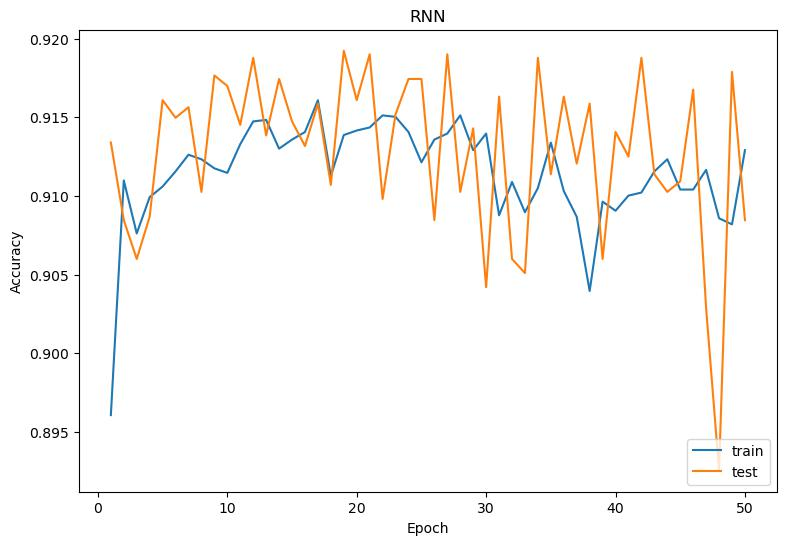
\includegraphics[width=\linewidth]{../figure/RNN_Accuracy.jpg}
    \end{minipage}
    \begin{minipage}{.43\linewidth}
        \centering
        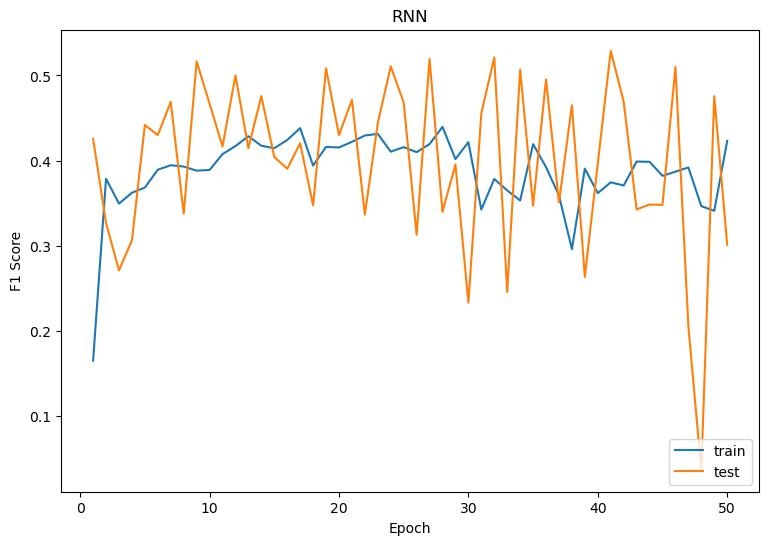
\includegraphics[width=\linewidth]{../figure/RNN_F1.jpg}
    \end{minipage}

    \begin{minipage}{.48\linewidth}
        \centering
        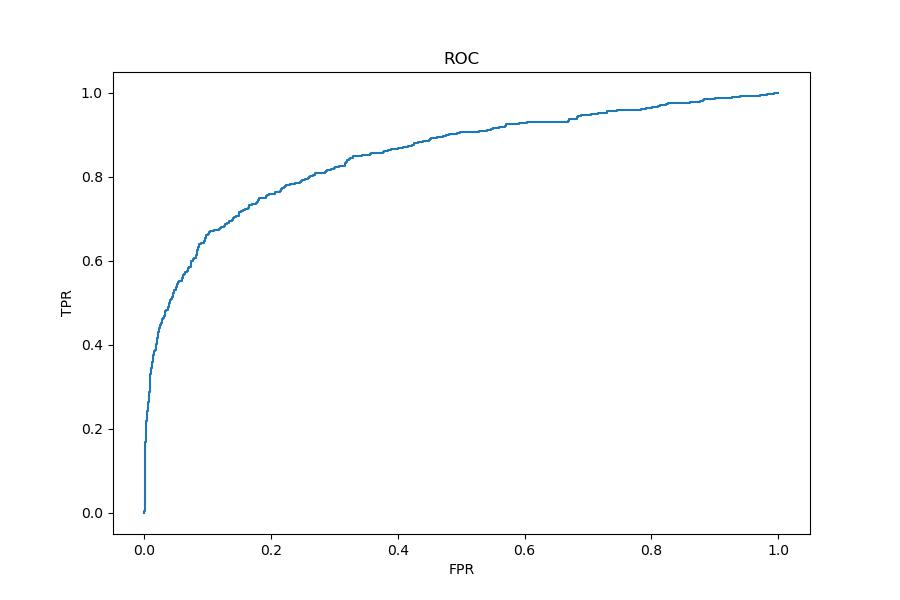
\includegraphics[width=\linewidth]{../figure/RNN_ROC.jpg}
    \end{minipage}
    \begin{minipage}{.48    \linewidth}
        \centering
        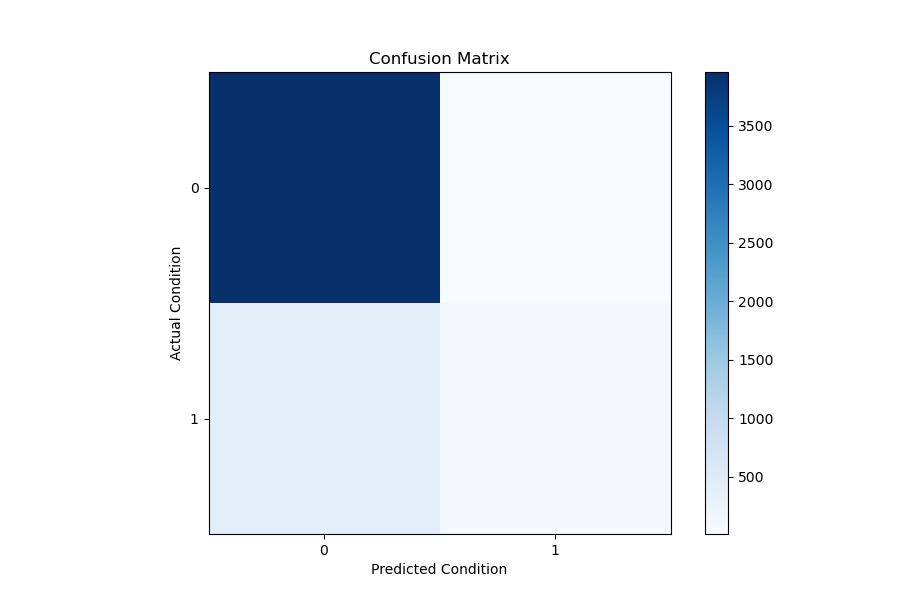
\includegraphics[width=\linewidth]{../figure/RNN_Confusion.jpg}
    \end{minipage}
    \caption{RNN}
\end{figure}

\begin{figure}[h]
    \centering
    \begin{minipage}{.43\linewidth}
        \centering
        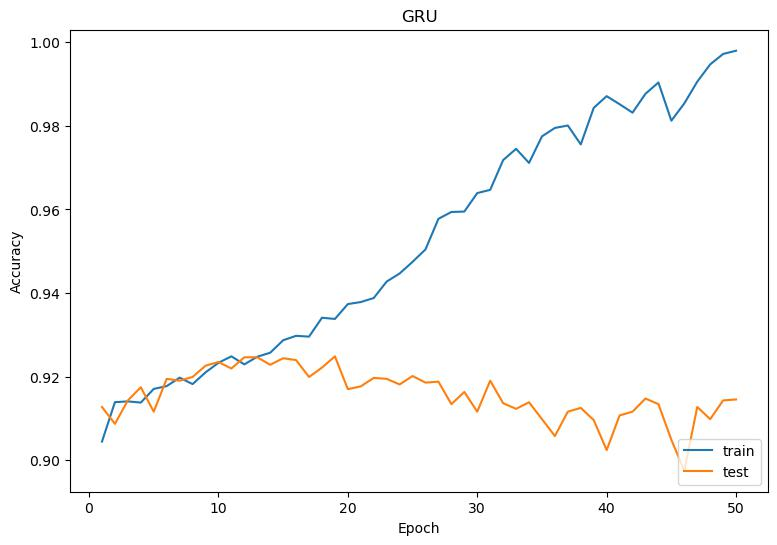
\includegraphics[width=\linewidth]{../figure/GRU_Accuracy.jpg}
    \end{minipage}
    \begin{minipage}{.43\linewidth}
        \centering
        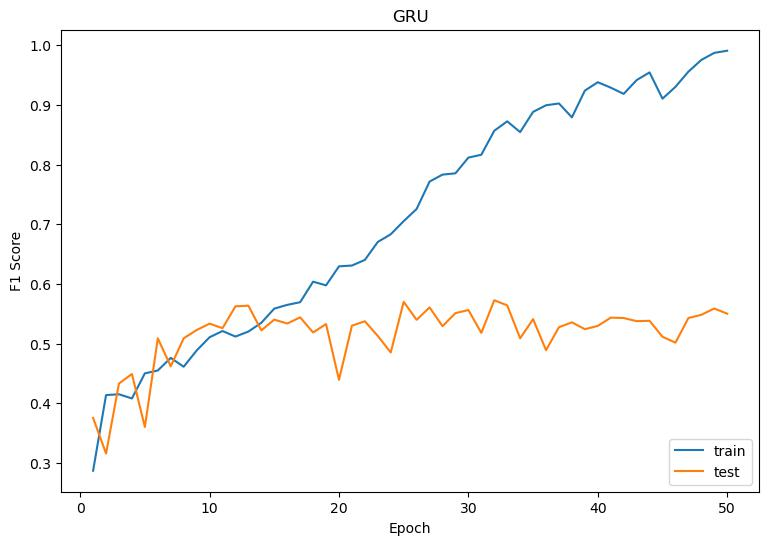
\includegraphics[width=\linewidth]{../figure/GRU_F1.jpg}
    \end{minipage}
    
    \begin{minipage}{.48\linewidth}
        \centering
        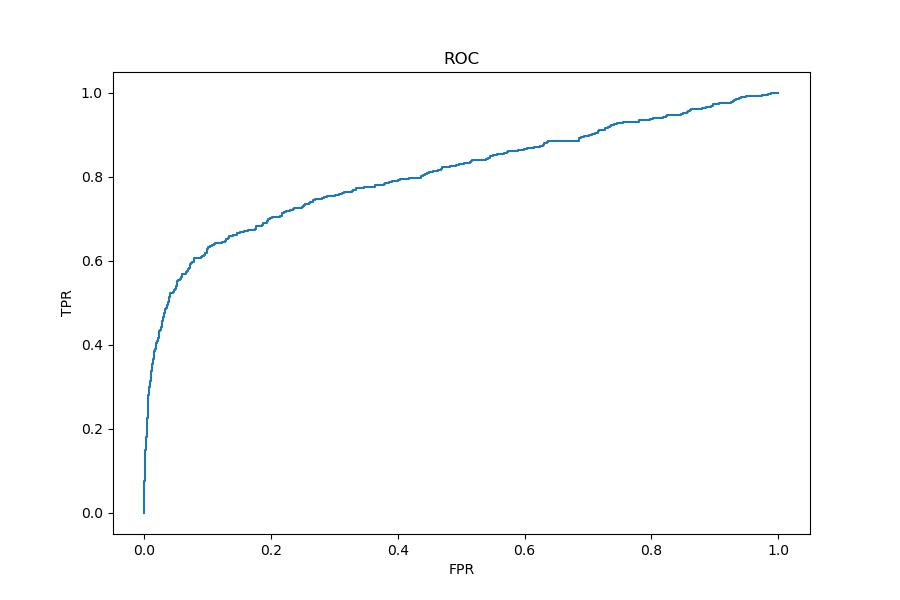
\includegraphics[width=\linewidth]{../figure/GRU_ROC.jpg}
    \end{minipage}
    \begin{minipage}{.48\linewidth}
        \centering
        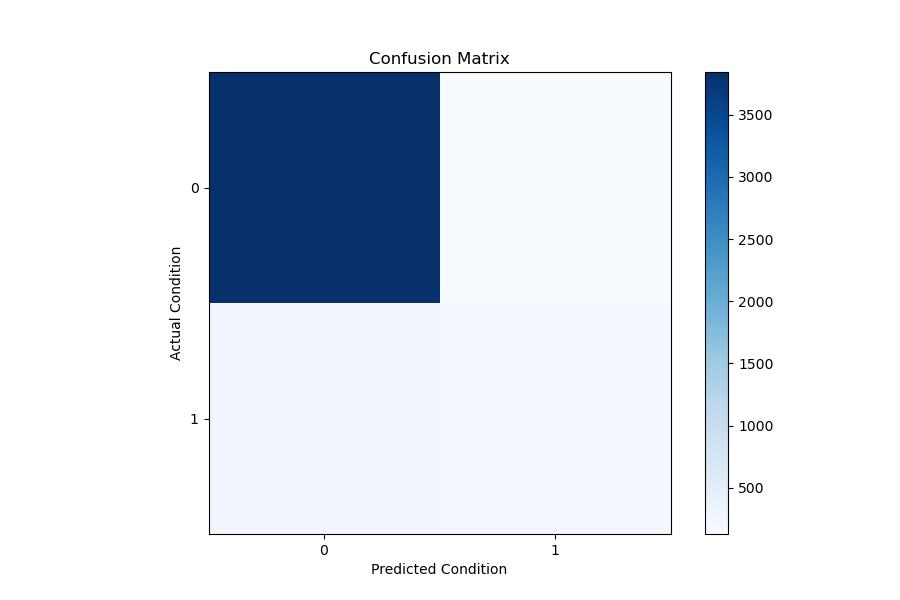
\includegraphics[width=\linewidth]{../figure/GRU_Confusion.jpg}
    \end{minipage}
    \caption{GRU(torch.nn)}
\end{figure}

\begin{figure}[h]
    \centering
    \begin{minipage}{.43\linewidth}
        \centering
        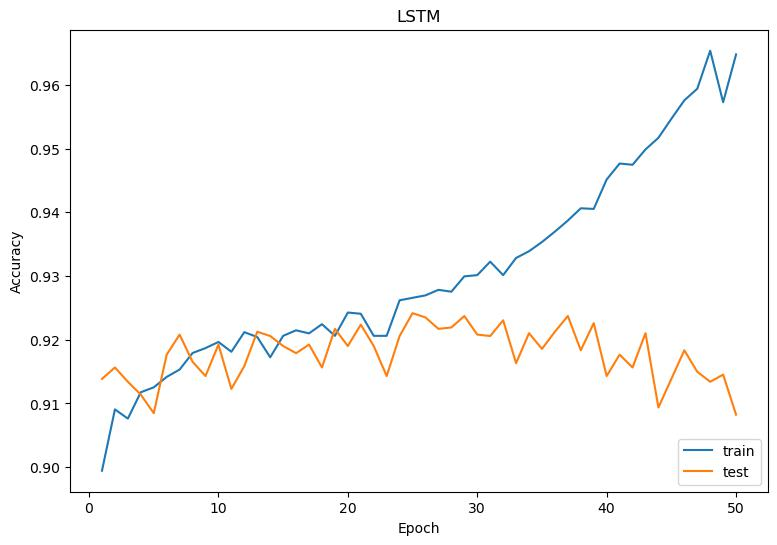
\includegraphics[width=\linewidth]{../figure/LSTM_Accuracy.jpg}
    \end{minipage}
    \begin{minipage}{.43\linewidth}
        \centering
        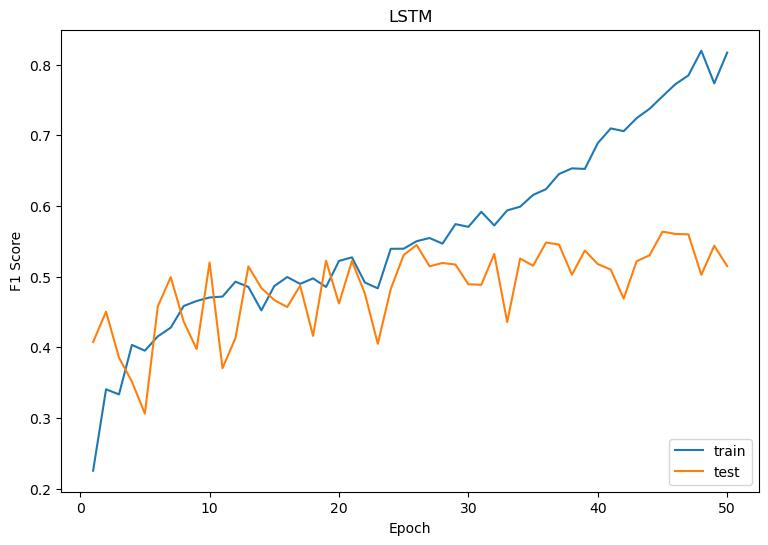
\includegraphics[width=\linewidth]{../figure/LSTM_F1.jpg}
    \end{minipage}

    \begin{minipage}{.48\linewidth}
        \centering
        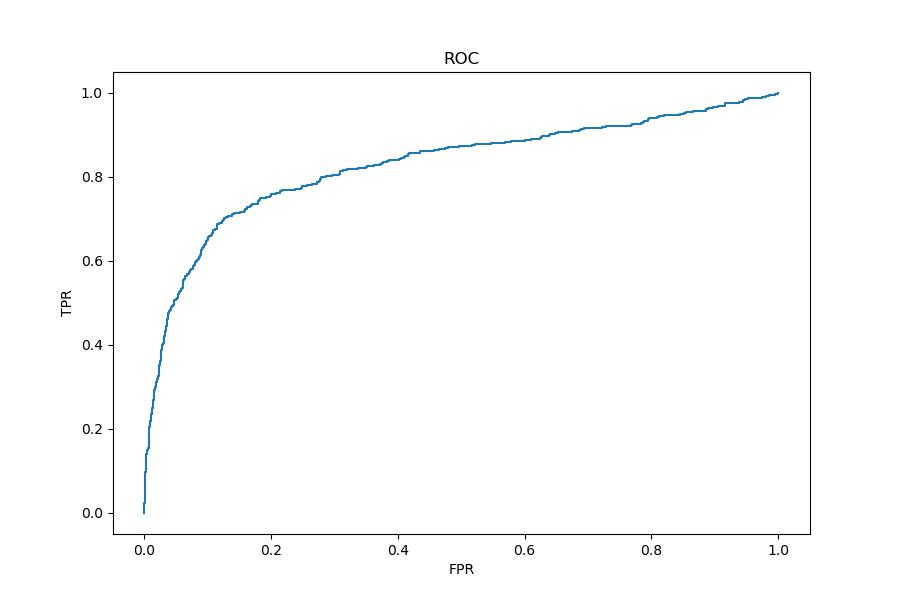
\includegraphics[width=\linewidth]{../figure/LSTM_ROC.jpg}
    \end{minipage}
    \begin{minipage}{.48    \linewidth}
        \centering
        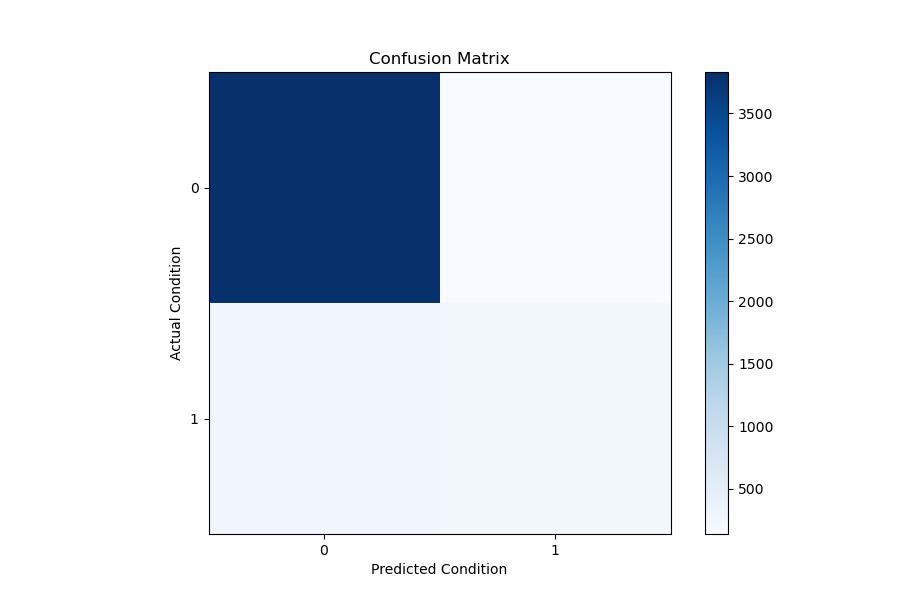
\includegraphics[width=\linewidth]{../figure/LSTM_Confusion.jpg}
    \end{minipage}
    \caption{LSTM}
\end{figure}

\subsection{GRU}
\subsubsection{机器学习库函数}
我们使用torch.nn.GRU作为模型对数据集进行训练。可以发现,GRU对训练集数据的建模能力强,可以在50个epoch处达到极高的Accuracy和F1 Score。但是可以发现,虽然测试集的F1 Score随着epoch而上升,但是其最高值仍然在0.58左右。这说明模型存在过拟合,且recall较低。这从ROC曲线课混淆矩阵中也能看出。

\subsubsection{人工实现}
对于人工实现的GRU,我们使用torch中提供的tensor乘法等方法进行模型的构建。可以发现,Accuracy和F1 Score的变化趋势与调用机器学习库函数的结果相同,但是训练速度慢于调用库函数的场景。这是因为库函数中使用了多种加速和优化方法,而我们的人工实现则并没有使用。同时,可以发现事实上测试集的F1 Score与调用库函数的结果相似。这可能是因为更少的优化方法反而带来了更少的过拟合。
\begin{figure}[h]
    \centering
    \begin{minipage}{.43\linewidth}
        \centering
        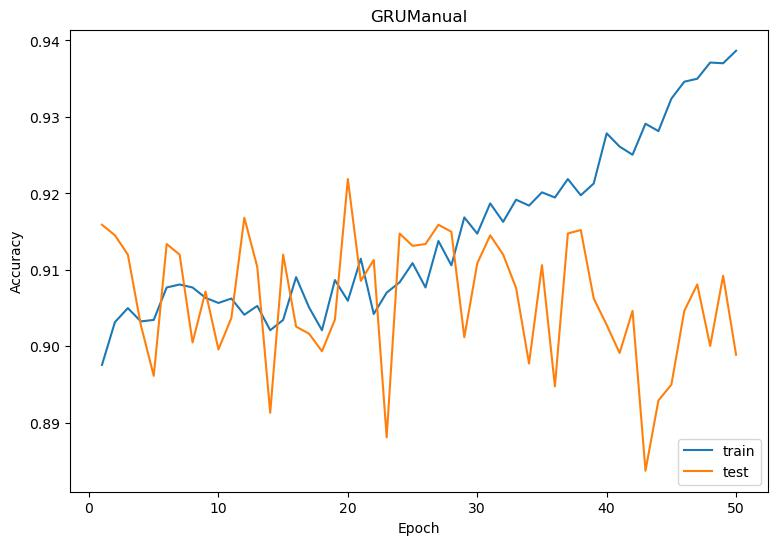
\includegraphics[width=\linewidth]{../figure/GRUManual_Accuracy.jpg}
    \end{minipage}
    \begin{minipage}{.43\linewidth}
        \centering
        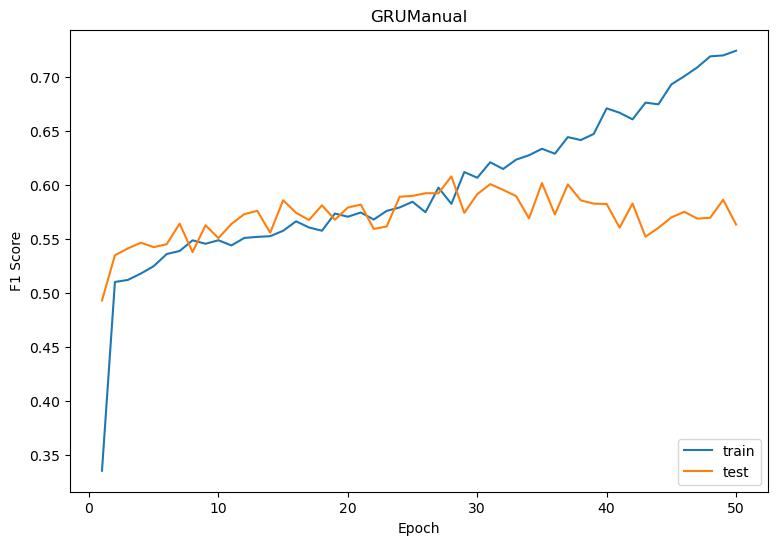
\includegraphics[width=\linewidth]{../figure/GRUManual_F1.jpg}
    \end{minipage}

    \begin{minipage}{.48\linewidth}
        \centering
        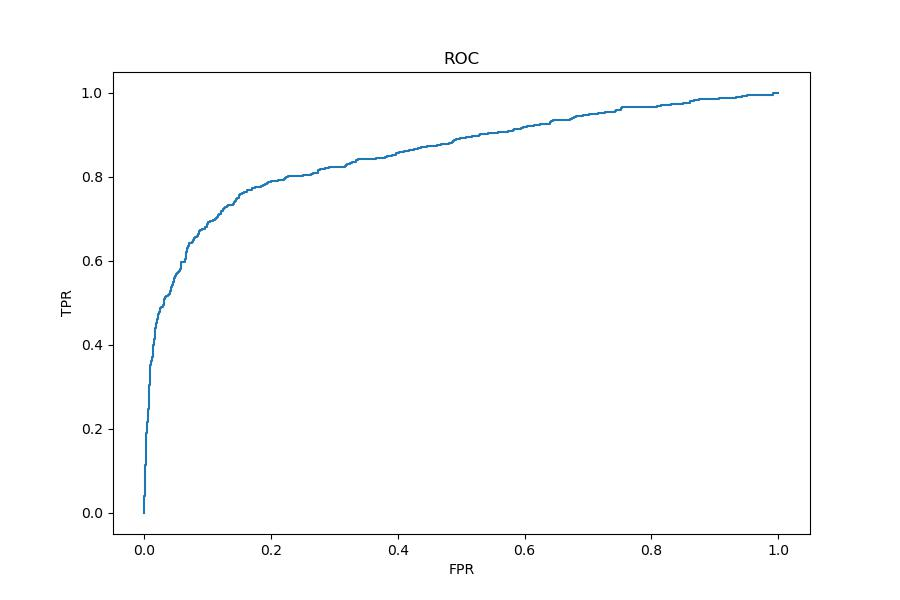
\includegraphics[width=\linewidth]{../figure/GRUManual_ROC.jpg}
    \end{minipage}
    \begin{minipage}{.48    \linewidth}
        \centering
        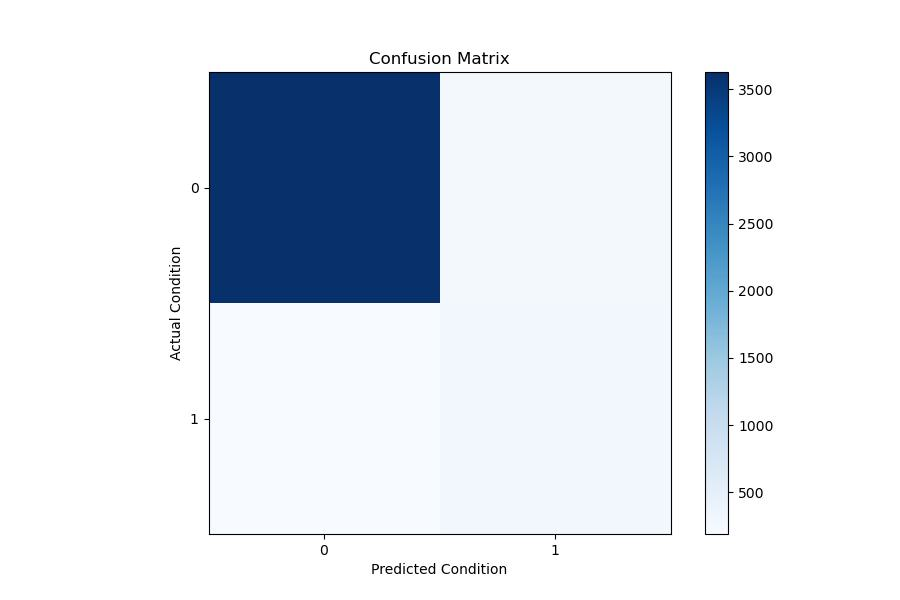
\includegraphics[width=\linewidth]{../figure/GRUManual_Confusion.jpg}
    \end{minipage}
    \caption{GRU(人工实现)}
\end{figure}

\subsection{LSTM}
我们使用torch.nn.LSTM作为模型对数据集进行训练。对于LSTM,可以发现其训练速度也略慢于GRU。同时,其F1 Score与GRU相近,且优于传统RNN。这说明,LSTM在未知长度的时间序列建模任务上仍然有优势,且过拟合的现象相较于GRU并没有那么严重。但是LSTM在Recall上的表现仍然不佳,这可以从混淆矩阵中看出。

\newpage
\section{小结}
本次大作业中,我们首先对病人的数据集进行清洗,通过规范化数据使得所有数据的区间落入$[0,1]$并使得所有病人的生命体征数据序列等长。

而后,我们使用传统RNN、GRU(torch.nn版本与人工实现版本)和LSTM对数据集进行建模,并对测试集进行预测。实验结果表明,LSTM和GRU在训练效果上优于传统RNN,而人工实现的GRU则与torch.nn版本相比有着相似的训练趋势和更慢的训练速度。这些都是符合直觉的结果。

同时可以发现,预测结果拥有极高Accuracy和中等F1 Score。这和数据集的质量以及正负标签比例都有关。
\end{document}